\chapter{Подавление артефактов, вызванных наличием сильнопоглощающих включений} \label{chapt2}
\section{Причины возникновения артефактов}
\label{sect_2_0}
Здесь надо подробно описать используему модель возникновения артефактов из-за сильнопоглощающих включений.
Причина этому - количество фотонов, проходящих через металлические вставки, недостаточно для возбуждения электронов на чувствительном элементе детектора (на матрице).
В резульате измерения в этих пикселях детектора записаны как 0, то есть излучение сюда не пришло.
В реальности же, по этому 0 можно сказать только лишь то, что излучения туда пришло меньше чем порог активации пикселя.
Таким образом, в пикселях с 0 значением пришедшей энергии правильно ввести ограничения-неравенства.
При этом если использовать алгебраический подход, мы получаем задачу условной квадратичной минимизации, или квадратичного программирования.

\section{Компьютерная томография как задача квадратичного программирования} \label{sect_2_1}

Для решения этой задачи предлагается использовать численную реализацию алгоритма interior-point-convex из MATLAB (quadprog) \todo{найти нормальну ссылку на алгоритм и матлаб}

\section{Описание образца} \label{sect_2_1_1}
\begin{figure}
  \centering
  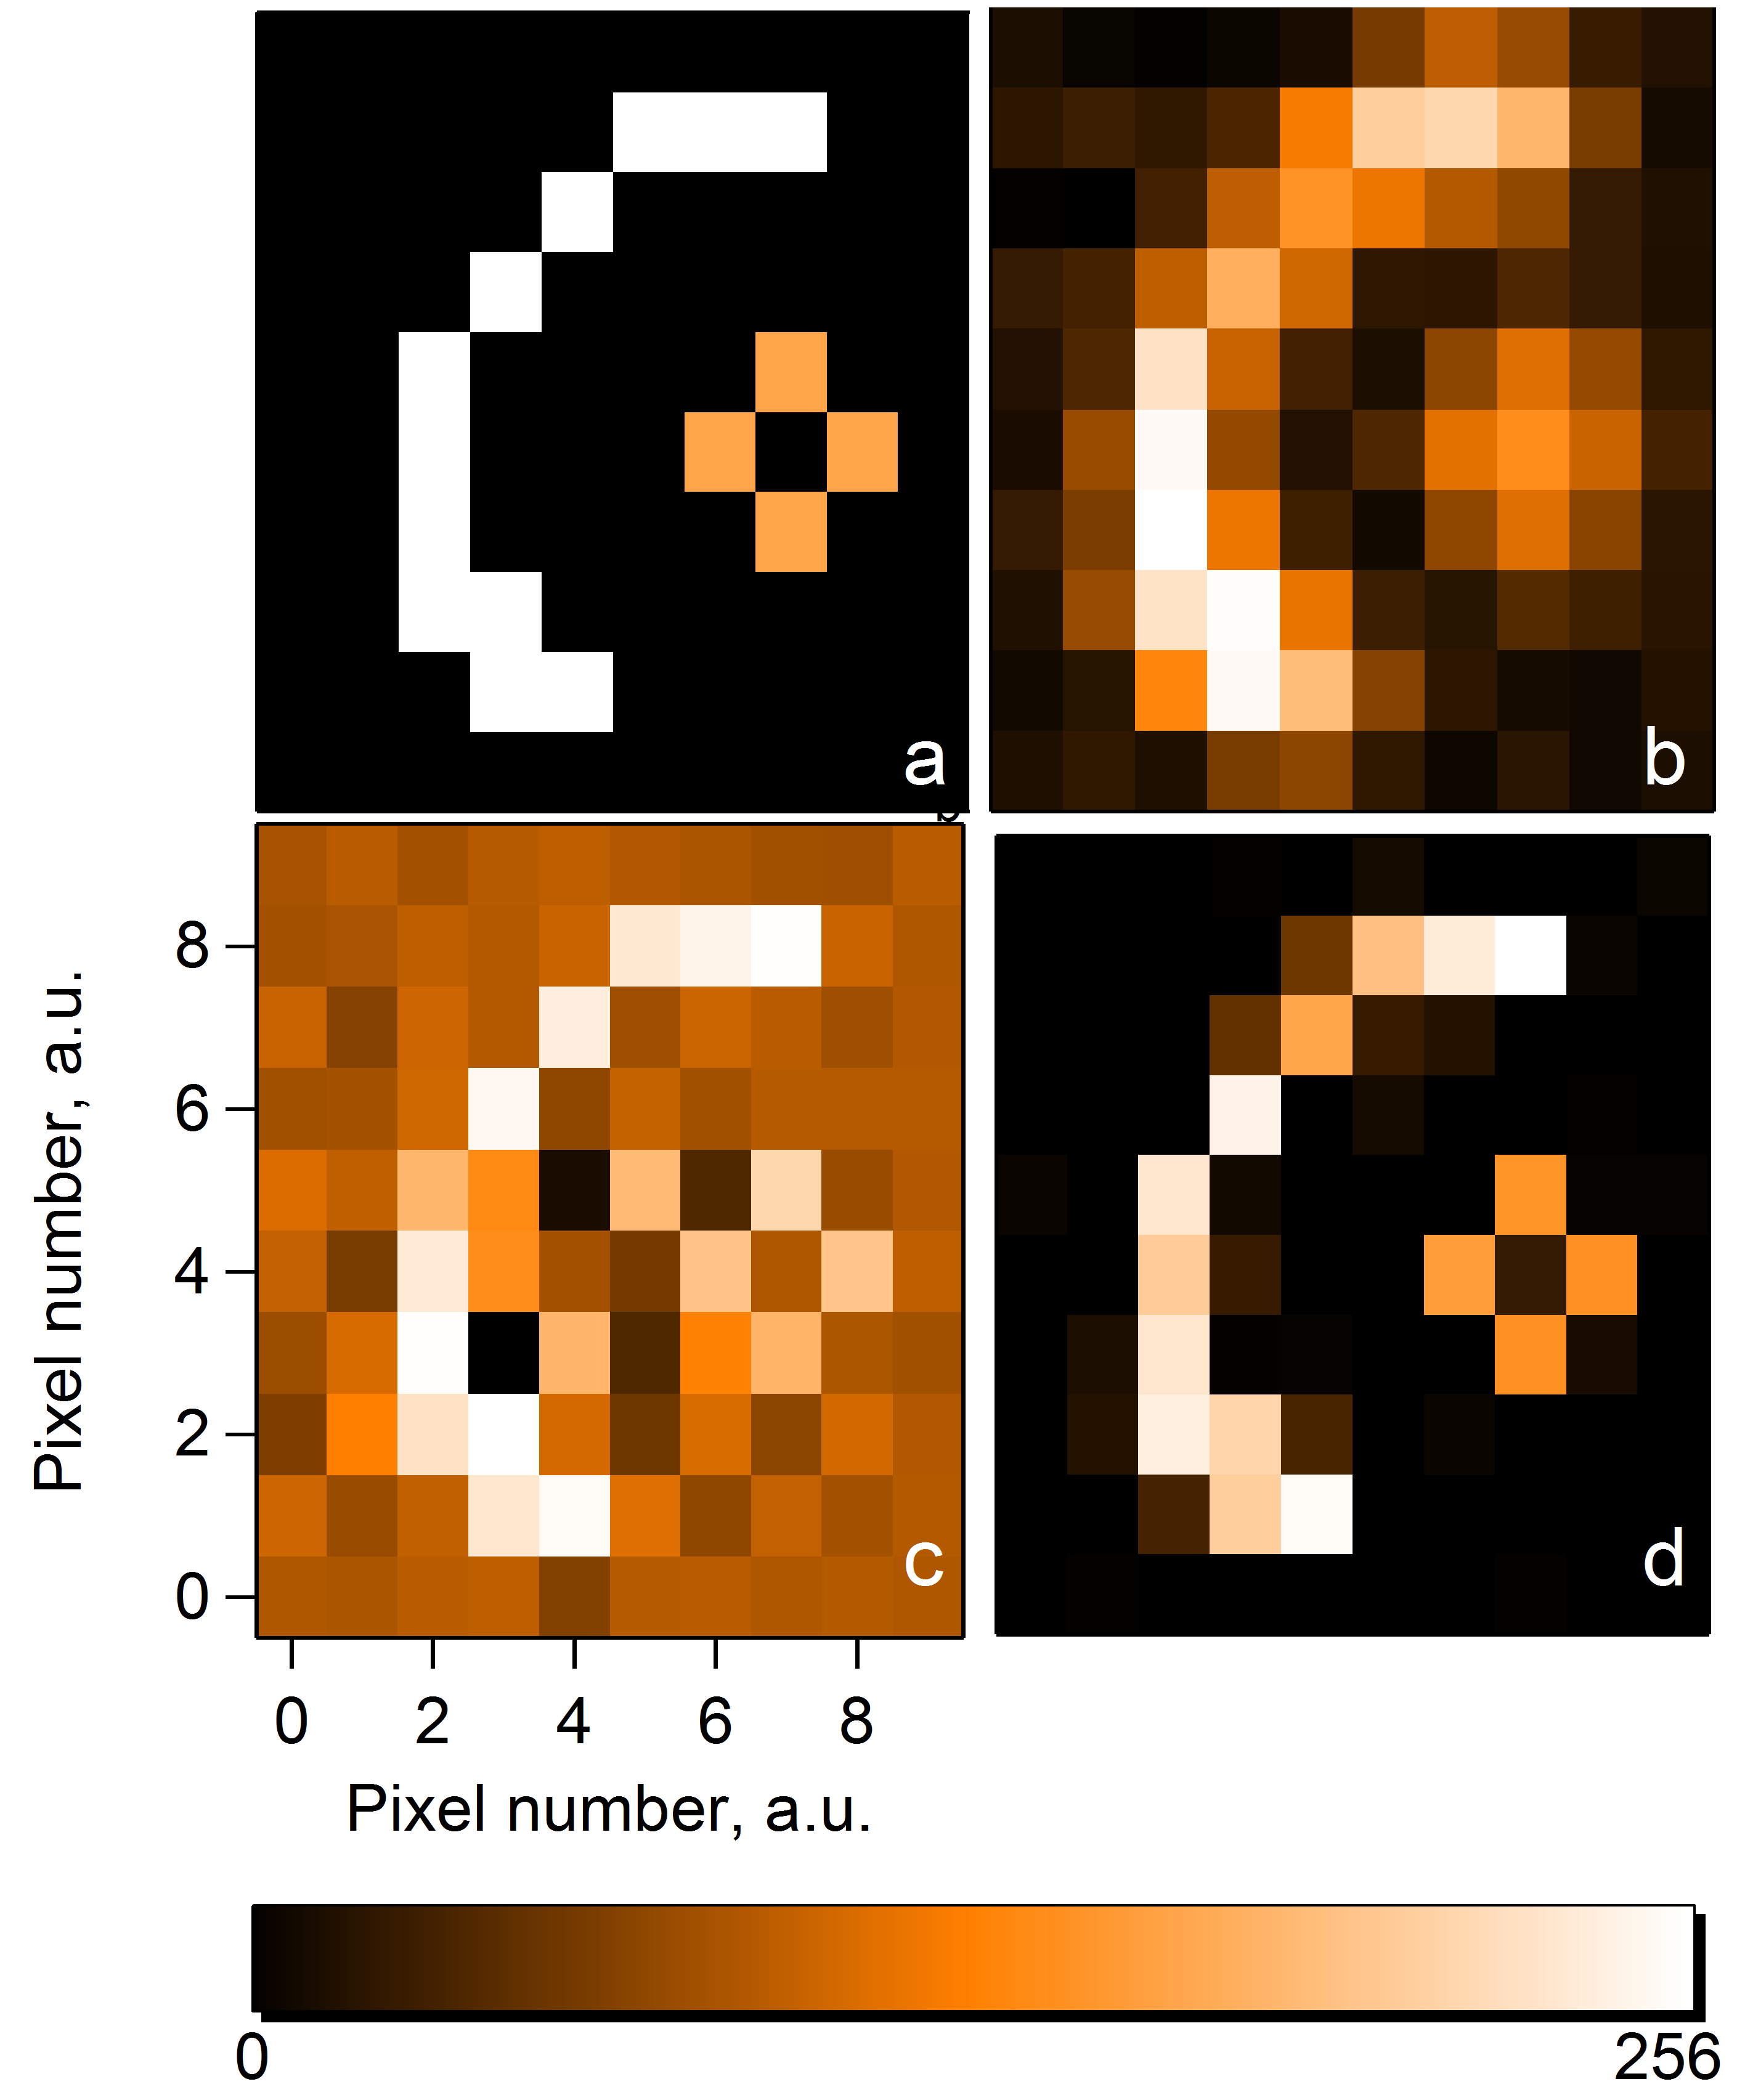
\includegraphics[width=0.7\textwidth]{part2_img/quadprog}
  \caption{Слева сверху - фантом использовавшийся для симуляций. Справа сверху - результат восстановления FBP. Слева снизу - результат восстановления квадратичным программированием без ограничений-неравенств. Справа снизу - результат восстановление квадратичным программированием с ограничениями-неравенствами (предложенный метод)}
  \label{im:quadprog}
\end{figure}

Для симуляции использовался фантом, изображенный на рисунке \ref{im:quadprog}a).
Это распределение вещества в сечении 10х10 пикселей, состоящее из двух объектов: скобки с высоким коэффициентом поглощения и крестика с нормальным уровнем поглощения.
Сгенерированная синограмма обрезалась по заданному значению порога, эмитируя эффект металлических включений.
Таким образом, была расчитана матрица проекции $\omega$, такая, что проеция $P = \omega \mu$ происходила по закону:

\begin{equation}
\label{eq:quadprog_projection}
P_j = 
\begin{cases}
\sum_i \mu_{i}\omega_{ij} , & \mbox{если} \mu_{i}\omega_{ij} < \mbox{порог} \\
\mbox{порог}, & \mbox{иначе}
\end{cases}
\end{equation}

, где $i$ - номер пикселя распределения, $j$ - номер луче проекции, порог подбирался таким образом, чтобы обрезать максимумы синограммы.
Значение порога было = 800, размер пикселя был 1х1.
Значение сильнопоглощающего включение было 256.
При расчете синограммы использовалось 35 проецкионых углов, равномерно распределенных в интервале от 0 до 180 градусов.

\todo{вставить синограмму}

На рисунке \ref{im:quadprog}b представлено восстановление полученной синограммы методом свертки и обратной проекции. 
Целью данного подраздела является улучшение данного восстановения методом квадратичного программирования.

Задача квадратичного программирования для воссатновления компьютерной томографии может быть сформулирована как 

\begin{equation}
  \label{eq:quadprog_eq}
  \begin{cases}
  \Norm{P^{\textup{изм.}} - P(\mu)} \rightarrow \min_{\mu} & w.r.t \\
  \sum_i \mu_{i} \omega_{ij} = P_j, & j = 1 \dots 35
  \end{cases}
\end{equation}

То есть условная минимизация с ограничениями типа равенства.
Результаты восстановления с помощью решения задачи (\ref{eq:quadprog_eq}) представлены на рисунке \ref{im:quadprog}с.

Следующим шагом в развитии этого метода восстановления является учет ограничений типа неравенства (\ref{eq:quadprog_projection}), учитывающих эффект сильного поглощения металлов.
задача (\ref{eq:quadprog_eq}) переходит в следующую:
\begin{equation}
  \label{eq:quadprog_ineq}
  \begin{cases}
  \Norm{P^{\textup{изм.}} - P(\mu)} \rightarrow \min_{\mu} & w.r.t \\
  \sum_i \mu_{i} \omega_{ij} = P_j, & \mbox{если} P^{\textup{изм.}}_j < \mbox{порог} \\
  \sum_i \mu_{i} \omega_{ij} > \mbox{порог}, & \mbox{если} P^{\textup{изм.}}_j = \mbox{порог}
  \end{cases}
\end{equation}

Восстановление с помощью решения (\ref{eq:quadprog_ineq}) изображено на рисунке \ref{im:quadprog}d.
Как видно из рисунка, квадратичное программирование с условиями неравенствами обеспечивает лучшее восстановление границ и интенсивностей исходного фантома. 
Значения интенсивностей на разных частях восстановленых фантомов приведены в таблице \ref{tb:quadprog_res}:

\begin{table}[h]
\label{tb:quadprog_res}
\centering
\begin{tabular}{ r| c| c| c| c|}
 & \ref{im:quadprog}a & \ref{im:quadprog}b & \ref{im:quadprog}c & \ref{im:quadprog}d \\ \hline
скобка & $255 \pm 0$ & $146 \pm 25$ & $233 \pm 30$ & $225 \pm 26$ \\ \hline
крест & $164 \pm 0$ & $69 \pm 3.6$ & $170 \pm 19.5$ & $151 \pm 5.2$ \\ \hline
\end{tabular}
\caption{Средние значения и стандартное отклонение интенсивностей в разных областях исследуемого фантома}
\end{table}

Так же можно заметить, что использование квадратичного программирование с ограничениями типа неравенство обеспечивет лучшие значения интенсивностей с меньшим значением отклонения.


\section{Результаты} \label{sect_2_1_2}

\todo{текст ECMS\_2015}

\section{Мягкие ограничения на неравенства} \label{sect_2_2}

In this paper, we improve the results achieved in \cite{chukalinaway}. First, we provide a robust to noise and admissible to efficient optimization methods way to express the inequalities introduced in \cite{chukalinaway}. Second, we evaluate the method's performance on a simulated phantom data. The phantom data was simulated to remind a teeth with a metal object. And finally we evaluate the gain we get using the information in the inequalities against not using it at all.

The sections are organized as follows. Section \ref{s-approach} outlines the detail our approach to solve the problem. In Section \ref{s-phantom} the simulated phantom is presented. The obtained results are discussed in Section \ref{s-results}. Section \ref{s-conclusion} then concludes the whole paper.

% \section{Описание подхода}
\label{s-approach}
Let us denote the distribution of the attenuation coefficient in the reconstructed volume with $x \in \mathbb{R}^m$. The $p \in \mathbb{R}^n$ denotes the projection data detected during a scan. According to Beer-Lambert law the energy, detected at the detector cell, corresponding to $i$-th ray is expressed by the formula $p_i = I_0 * \exp(-a_i^T x)$, where $I_0$ is the source intensity, and $a_i$ is the row of the projection matrix $A$ corresponding to the $i$-th ray. A standard approach to find $x$ from the projection data is to take a logarithm and solve the linear system of equations: $Ax = r$, where
$r_i = \log(I_0) - \log(p_i)$. A standard way to get robust to noise reconstruction here is to use linear least squares:
\begin{equation} \label{eq:lls}
  \Norm{Ax - r}^2 \to \min\limits_{x}.
\end{equation}

Metal streak artifacts are caused mainly by photon starvation and noise. Mathematically it corresponds to the rays where $p_i$ is small or even zero. In latter case the logarithm is not defined and the simples way is just to ignore those rays solving instead of \eqref{eq:lls}:
\begin{equation}
  \label{eq:mask-lls}
  \Norm{P(Ax - r)}^2 \to \min\limits_{x},
\end{equation}
where matrix $P$ takes only those coordinates of a vector, at which $p_i \neq 0$. More precisely,
$$
P_{i,j} = \begin{cases}
  1, \quad\text{if $i = j$ and $p_i > 0$} \\
  0, \quad\text{otherwise}
  \end{cases}.
$$

It was suggested in \cite{chukalinaway} that even such problematic rays provide us with some information, namely that the weighted sum along such a ray has lower bound $a_i^T x > B$, for some suitable value of $B$ (for example, $B = \log I_0$), and we can use this information in a form of linear inequality constraints, solving the linear system with linear least squares approach:
\begin{equation}
  ||P(Ax - r)||^2 \to \min\limits_x, \quad\textrm{s.t. }  QAx \ge B,
\end{equation}
where $Q$ takes only those coordinates of a vector at which $p_i = 0$, opposite to the matrix $P$. Basically, $Q = E - P$, where $E$ is identity matrix.

This constraints being mathematically correct, are tight and are not robust against the noise in the projection data. Instead of tight constraints we propuse to use a soft version provided with a quadratic penalty method \cite{nocedal2006numerical} instead:
\begin{equation}
  \label{eq:soft-ineq}
  ||P(Ax - r)||^2 + \alpha ||[QAx - B]^-||^2 \to \min\limits_x,
\end{equation}
where $[y]^- = \min\{0, y\}$.

This functional provides a soft way to enforce the inequalities on the variables, but also allows to handle noise effects more smoothly. We can regulate the effect of that smoothing by manipulating $\alpha$: the greater $\alpha$ is tighter the effect of inequalities is.

The objective function \eqref{eq:soft-ineq} is convex and differentiable. We can effectively minimize it with Conjugate Gratient method (we used the implementation of this method, provided by the Python package \cite{scipy}). To speed-up computation of forward and backward tomographic projection operators we used ASTRA Toolbox \cite{palenstijn2011performance, van2015astra} which performs efficient evaluation of such operators on GPU.
\begin{figure}[h]
  \centering
  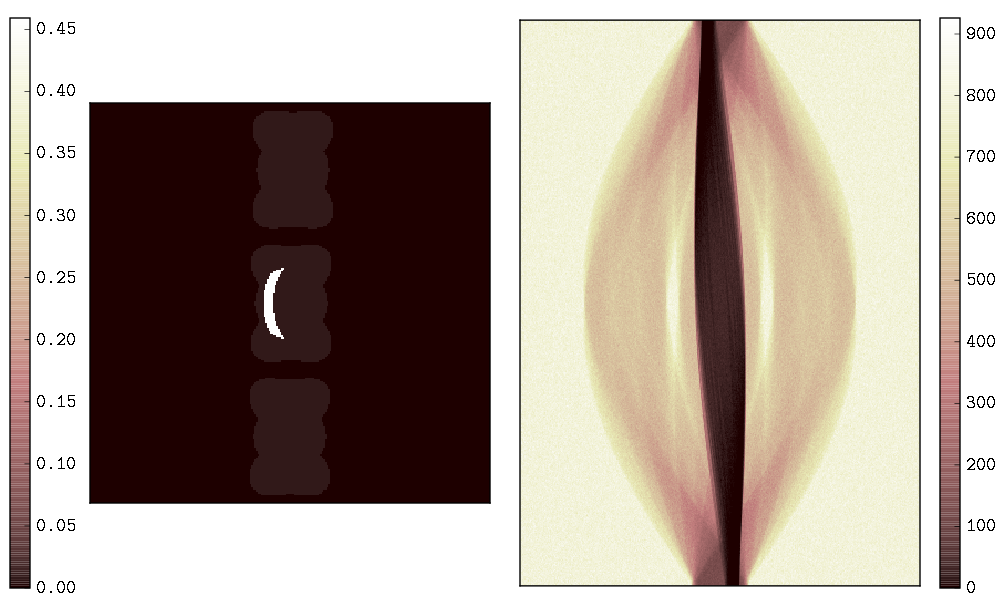
\includegraphics[scale=0.45]{part2_img/phantom-and-projection}
  \caption{The phantom (left) and its projection at $I_0 = 10^3$ photons (right).}
  \label{phantom-and-projection}
\end{figure}

\section{Описание образца}
\label{s-phantom}
To simulate the sinogram in $55$keV monochromatic mode we used a phantom imitating three teeth. Middle tooth contains titanium include imitating an implant (fig. \ref{phantom-and-projection}, left image). Pixel size is $0.005$cm. 2D field view size is $256 \times 256$ pixels. We used the XRayLib library \cite{brunetti2004library, schoonjans2011xraylib} to calculate the X-ray attenuation in each pixel for chosen energy. The sinogram (fig. \ref{phantom-and-projection}, right image) was calculated in a parallel scheme. We used $512$ rotation angles uniformly distributed in the interval $[0, \pi)$. The number of the detector cells is $362$, so that the diagonal of the phantom is projected on the detector without loosing any information. Such geometry choice allowed us to ignore the uniqueness of the solution issues which are related to the null-space of the projection operator and are ususally dealt with some sort of regularization techniques.

\section{Результаты}
\label{s-results}
To study the proposed approach we generated projections for different source intensities and draw several samples of Poisson noise at each source intensity.

For each projection we reconstructed the volume using Missing Data Least Squares \eqref{eq:mask-lss} and proposed Soft Inequalities Least Squares \eqref{eq:soft-ineq} approaches. The value of $\alpha$ was chosen to be equal to $50$.. The reconstructed volume was then compared to the original phantom and Mean Square Error was compute for such a pair.

In the figure \ref{sample} we can see an example of such reconstructions. In absence of the information encoded in the inequalities the metal artifacts are presented and there is a strong shadow in the cental tooth, while in the left image, reconstructed with Soft Inequalities approach those artifacts are significantly reduced.
\begin{figure}
  \centering
  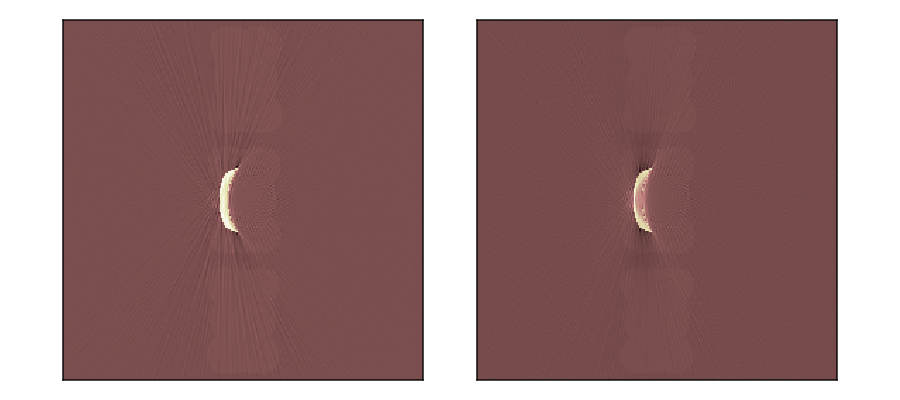
\includegraphics[scale=0.5]{part2_img/sample}
  \caption{Example of reconstruction with Soft Inequalities method (left)
    and Missing Data method (right).}
  \label{sample}
\end{figure}
In the figure \ref{error-plot} we can see the plot of MSE averaged over all the samples of noise for each noise level. The inequalities provide an improvement over ignoring such data at all noise levels.
\begin{figure}
  \centering
  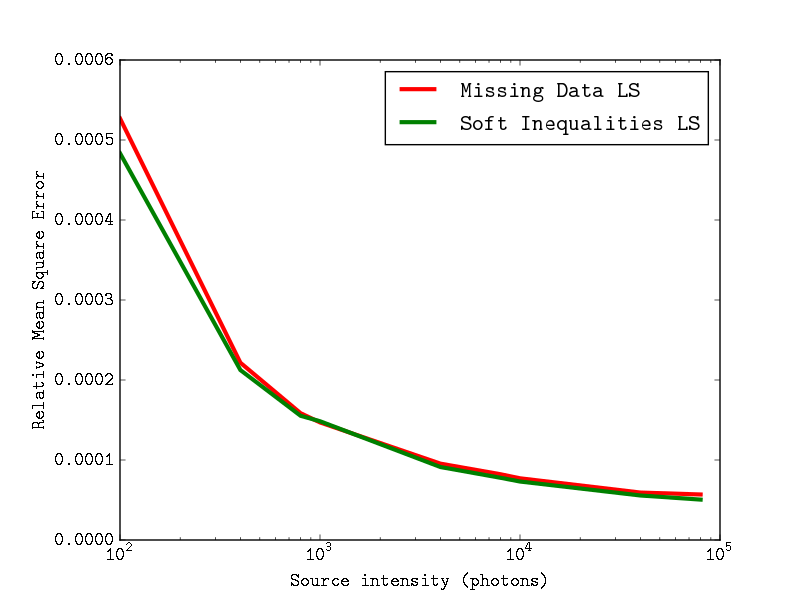
\includegraphics[scale=0.5]{part2_img/error-plot}
  \caption{The MSE value with respect to noise level.}
  \label{error-plot}
\end{figure}

\section{Выводы}
\label{s-conclusion}

Experiments shows that the information encoded in the inequalites, introduced in \cite{chukalinaway} carries a significant information which can be used to reduce metal-like artifacts in the reconstructions. We proposed a robust way to use this information in form of panaltized objective function. The proposed functional is suitable to be minimized with an efficient numerical algorithms enabling the approach to work on mid- and large-sized data. Proved to work, the method next should be deeper with respect to sensitivity to $\alpha$ and compared against the other approaches mentioned in the introduction. It is also seems possible to leave the penalty encoding the inequality constraints, replacing the least squares functional with more statistically suitable (for example, Poisson log-likelihood, used in MLEM) data fit functional.

\subsection{параметры моделирования и восстановления} \label{sect_2_3}
Параметры моделирования:
\begin{itemize}
  \item размером фантома (size, 65, 256),
  \item количеством углов проекции (n\_angles, 90, 512), 
  \item интенсивность пучка (i0, 1000)
  \item энергия пучка (45 кэв)
  \item форма фантома (три зуба и имплант-бумеранг)
  \item материалы фантома и импланта (Ca, Au)
  \item наличие импланта (в наличии)
  \item размер пикселя (0.05)
  \item наличием шума при прокеции, распределением шума (есть пуассоновский шум)
\end{itemize}

Параметры восстановления:
\begin{itemize}
  \item итераций 200 (где-то 300)
  \item $\alpha$ 30 и 300
\end{itemize}